\documentclass[conference]{IEEEtran}
\usepackage[utf8]{inputenc}
\usepackage[german]{babel}

\usepackage{graphicx}
\graphicspath{figures/}

\makeatletter
\let\@copyrightspace\relax
\makeatother

\begin{document}

\title{MAC Authentication Bypass (MAB)\\ in Industrie 4.0}
\author{
	Umut-Vural Mitiler\\
	u.mitiler@stud.hs-wismar.de
	\and
	Fakultät für Ingenieurwissenschaften\\
	Hochschule Wismar\\
	Master IT-Sicherheit und Forensik\\
	Industrial Security\\
	Gruppe FFM-08
	\and
	David Schunke\\
	d.schunke@stud.hs-wismar.de
}

\maketitle

\thispagestyle{plain}
\pagestyle{plain}

%

\begin{abstract}
Eine kurze Beschreibung des Papers, worum gehts, was wird erklärt, was ist das Resultat.
\end{abstract}

\vspace{1em}

\begin{IEEEkeywords}
MAC Authentication Bypass, MAB, IEEE802.1X, dot1x, Network Access Control, NAC, Industrie 4.0
\end{IEEEkeywords}

%

\section{Einleitung}
Grundsätzliche Motviation für das Thema, was ist Industrie 4.0 und was ist NAC\\

Die fortschreitende Vernetzung von IT Systemen bahnt sich ihren weg durch alle Bereiche unseres Lebens. Während ständige Vernetzung im Privaten- sowie Dienstleistungsumfeld heute alltäglich für uns sind, ist in der Industrie ein solcher Grad an Vernetzung noch nicht angekommen. So sind häufig im industriellen Umfeld noch Maschinen oder Systeme eingesetzt, welche aufgrund ihres Alters gar keine Vernetzung und Kommunikation erlauben, als auch existierende Vernetzungen lediglich für eine einfachste Form der Kommunikation, wie z.B. Systemüberwachung, eingesetzt.\\

Industrie 4.0 stellt die aktuellste und vierte Stufe der industriellen Revolution dar. Nachdem die erste industrielle Revolution durch die Mechanisierung von Arbeitsprozessen, die zweite industrielle Revolution durch den Einsatz technischer Hilfsmittel zur Massenproduktion, und die dritte industrielle Revolution erste digitale Hilfsmittel zur Automatisierung geprägt waren, werden in der vierten industriellen Revolution alle Komponenten digitalisiert, vollumfänglich vernetzt als auch mit Intelligenz versehen, sodass diese Komponenten teils vollautonom dezentrale Entscheidungen treffen und untereinander Kommunizieren können. Der Mensch interagiert nur noch eingeschränkt und teilweise über neuartige Schnittstellen (human-computer-interfaces, HCI) mit den Systemen, um diese z.B. bei Konflikten oder benötigten Entscheidungen anzuleiten. Solche Systeme werden Cyberphysische Systeme (CPS) genannt und bilden das Rückgrat der Industrie 4.0.\\
% TODO Referenz zu den Stufen, HCI, CPS %

Mit Vernetzung und Kommunikation werden gleichzeitig solche Systeme allerdings auch stärker angreifbar und bedingen weitergehender Schutzmechanismen. Während in Office- oder User-Netzwerken
%TODO Footnote%
Technologien und Protokolle zur Absicherung der Kommunikation bereits lange zum Standard gehören, sind die in der Industrie noch häufig eingesetzten Systeme und Protokolle auf eine Absicherung noch nicht ausgelegt. Gefahren bilden hierbei u.A.
\renewcommand{\labelenumi}{\alph{enumi})}
\begin{enumerate}
	\item Industriespionage durch Abfangen von Kommunikation oder eindringen in Systeme (Angriff auf Vertraulichkeit)
	\item Manipulation von Kommunikation, z.B. Steuerbefehlen (Angriff auf die Integrität)
	\item Störung der (Echtzeit-)Kommunikation bis hin zu Denial-of-Service (DoS), sodass ein System komplett ausfällt (Angriff auf die Verfügbarkeit)
	\item Übernahme (Hijacking) von Systemen und missbräuchliche Verwendung oder Erpressung
\end{enumerate}

Die verschiedenen Gefahren stellen für die unterschiedlichen Zweige der Industrie auch unterschiedliche Schweregrade dar, sind jedoch in der Industrie 4.0 für alle Bereiche ein hochwichtiges Thema.\\

Ein zentraler Teil zur Absicherung gegen solche Gefahren besteht darin, wer überhaupt Zugang zu einem Netzwerk hat, analog zur Absicherung, wer überhaupt physisch Zugang zu einer Anlage hat. Hierbei haben sich in der Office-IT bereits unterschiedliche Strategien und Technologien gebildet, um eine Netzwerkzugangskontrolle (Network Access Acontrol, NAC)
% hier Footnote lieber oder so stehen lassen zu NAC? %
zu realisieren. Aufgrund des Alters vieler Systeme in der Industrie können diese Technologien allerdings nicht immer einfach übertragen werden, ohne Probleme in der Kompatibilität hervorzurufen, gleichzeitig aber auch nicht einfach durch neue Systeme ausgetauscht werden. Aus diesem Grund werden für solche Systeme Fallback-Lösungen benötigt, sodass diese Systeme trotz Netzwerkzugangskontrolle am Netzwerk und der Kommunikation teilnehmen können. Eine solche Technologie stellt das MAC Authentication Bypass (MAB) dar.

%

\section{Grundlagen}
Kurze technische Einführung

\subsection{dot1x}
Erklärung dot1x, was macht es, kurz technische Übersicht als Basis für MAB

\begin{figure}[hbt]
	\centering
	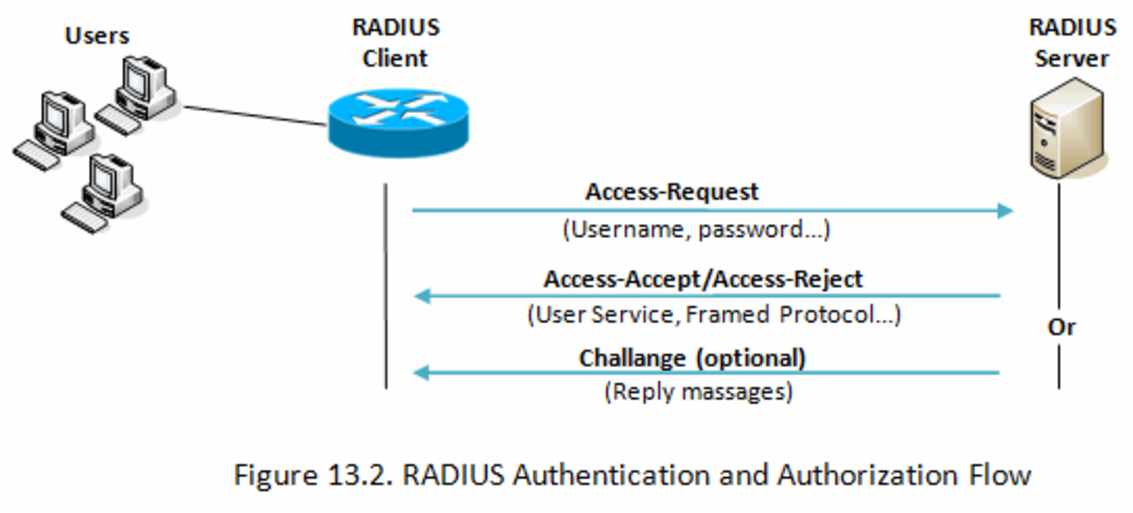
\includegraphics[width=8cm]{figures/Radius}
	\caption{Foobar \cite{einstein}}
\end{figure}

\subsection{Technische Umsetzung von MAB}
wie funktioniert MAB konkret, kurze technische Detailübersicht, was ist der Unterschied zu dot1x

%

\section{Praxiseinsatz}
NAC in der Praxis allgemein

\subsection{Heutiger Einsatz}
Wie wird MAB bereits jetzt eingesetzt\\
Fallback\\
Drucker, Telefone, IP-Phones, Kameras

\subsection{Relevanz in Industrie 4.0}
Hier kommt alles zur Relevanz von Industrie 4.0\\
Skalierbarkeit, Heterogene Landschaft, Einbindung von "Leichen"

%

\newpage

\section{Ergebnis}
Zusammenfassung was MAB macht, was es ist, wofür es nicht geeignet ist\\
Vorteile und Nutzen\\
Nachteile und Gefahren\\
Gegenmaßnahmen und Kombination mit anderen Technologien, wie z.B. IDS, usw.
\newline

Wie sieht die Zukunft von MAB aus

%

\bibliographystyle{IEEEtran}
\bibliography{references}

\end{document}